\subsection{Eficiencia de un algoritmo}

Con lo anterior, tenemos claro que una tarea se puede llevar a cabo mediante distintos algoritmos, entonces ¿cuál es el mejor?. Podemos asignarle una \textbf{medida} o un \textbf{tamaño} a un \textbf{caso} (o instancia). Y esto es subjetivo. Por ejemplo, para calcular la suma de dos números naturales $a$ y $b$ podemos asignar como medida del caso la cantidad de dígitos del máximo entre $a$ y $b$. Luego analizamos cuántas operaciones significativas se deben hacer en función de esa medida. Usando el algoritmo de adición básico:

\begin{center}
    \begin{tabular}{ccccccccccc|c}
            &   & 7 &   & 8 &   & 1 &   & 5 &   & 3 & $a$            \\
        $+$ &   & 3 &   & 7 &   & 4 &   & 2 &   & 9 & $b$            \\ \midrule
            & 1 &   & 1 &   & 0 &   & 0 &   & 1 &   & \text{llevo}   \\
         1  &   & 1 &   & 5 &   & 5 &   & 8 &   & 2 & $s$    
    \end{tabular}
\end{center}

\noindent entonces en el \textbf{peor de los casos}, si ambos números tienen $n$ dígitos, tendremos que ejecutar $n$ adiciones de números pequeños (es decir de un dígito) y una que otra adición más (cuando \textit{llevamos}). Nos guiamos por el peor de los casos.\marginnote{De igual manera, el algoritmo (usual) de la multiplicación de dos números naturales, si volvemos a tomar como medida de la instancia la cantidad de dígitos del mayor número, el algoritmo tiene eficiencia $n^2$. Ya que consideramos que las operaciones significativas son las multiplicaciones de un dígito.}


\begin{ejem}
    El siguiente algoritmo arroja la representación binaria del número $m$ dado en su     forma decimal.
    
    \begin{algoritmo}
    \caption{Representación binaria de un número en forma decimal}\label{alg:bin}
    \KwData{$y > 0$}
    \KwResult{$N_2$, representación binaria de $m$}
    $y \leftarrow N$\;
    $i \leftarrow 0$\;
    \If{$y = 0$}{
    \Return{$N_2 \leftarrow 0$}
    }
    \While{$y \neq 0$}{
        \eIf{$y$ \textup{es par}}{
            $r_i \leftarrow 0$\;}{
            $r_i \leftarrow 1$\;
            $y \leftarrow y-1$\;}
        $y \leftarrow y/2$\;
        $i \leftarrow i+1$\; 
    }
    $t \leftarrow i-1$\;
    \Return{$N_2 \leftarrow r_tr_{t-1}r_{t-2} \dots r_1r_0$}
    \end{algoritmo}
    
    \noindent el proceso es como se muestra a continuación, y termina cuando el cociente es cero
    
    \begin{gather*}
        N = 2 \cdot q_0 + r_0 \\
        q_0 = 2 \cdot q_1 + r_1 \\
        \vdots \\
        q_{t-2} = 2 \cdot q_{t-1} + r_{t-1} \\
        q_{t-1} = r_t \quad (q_i = 0)
    \end{gather*}
    
    \noindent luego la representación binaria es $r_tr_{t-1} \dots r_1r_0$. Si el tamaño de la instancia es la cantidad de dígitos de $m$\marginfootnote{En el Biggs, se consideran dos posibles medidas para el tamaño: el valor de $m$ como tal, o su cantidad de dígitos}, digamos
    
    \[
    m = x_{n-1}x_{n-2}\dots x_1x_0 \quad \text{en base 10}
    \]
    
    \noindent entonces $10^{n-1} < m \leq 10^n-1$, por lo que $n-1$ es la parte entera de $\log_{10}m$, por lo que el número $n$ de decimales en $m$ está dado por\marginnote{En el vídeo Nieto solo dice "aplicando logaritmo" en este paso. Esta explicación fue sacada directamente del libro (página 145).}
    
    \[
    n = \lfloor \log_{10}m + 1 \rfloor
    \]
    
    \noindent ahora, la operación más significativa es la división entre 2. ¿Cuántas veces?: pues $t+1$, que coincide con la cantidad de dígitos de la representación binaria. O sea, que tenemos
    
    \[
    t + 1 = \lfloor \log_2m \rfloor + 1 = \lfloor \log m / \log 2 \rfloor + 1 \quad \footnotemark
    \]\footnotetext{Se aplican propiedades de los logaritmos en este paso.}
    
    Así que $t+1$ en función de $n$ es aproximadamente $\frac{10}{3}n$. Sólo nos interesa el comportamiento de la eficiencia para valores grandes de $n$, por eso nos conformamos con una aproximación.
\end{ejem}

\subsection{Notación "$O$ grande"}

\begin{defn}    
    Dadas las funciones $f, g: \N \rightarrow \N$, decimos que $f$ es \ul{$O(g(n))$} si eventualmente
    
    \[
    f(n) \leq \lambda g(n)
    \]
    
    \noindent para algún $\lambda > 0$. Es decir, la desigualdad se cumple excepto para una cantidad finita de valores de $n$.
\end{defn}

\begin{ejem}
    Consideremos lo siguiente
    
    \[
    3n^3 + 20n^2 + 5n + 11 \leq (3 + 20 + 5 + 11)n^3 = 39n^3
    \]
    
    \noindent así que $f(n) = 3n^3 + 20n^2 + 5n + 11$ es $O(n^3)$. También $2^n + 3n^5 + 12n^4$ es $O(2^n)$.
\end{ejem}

\begin{nota} 
    Hay que tener presente lo siguiente:
    
    \begin{enumerate}
        \item Decir que $f(n)$ es $O(g(n))$ \textbf{no significa} que $f(n) = O(g(n))$ (esto ni sentido tiene).
        \item Si $f(n)$ es $O(g(n))$ y $h$ es una función que supera a $g$, entonces $f(n)$ también es $O(h(n))$. Por ejemplo, si $f(n)$ es $O(n^4)$, entonces también es $O(n^7)$. Pero la idea es buscar una opción óptima para $g$ cuando analizamos la eficiencia de algoritmos.
    \end{enumerate}
\end{nota}

\subsection{Comparar algoritmos}

Veamos, como ejemplo que se puede mejorar (respecto a la eficiencia) el algoritmo usual para calcular la $m$-ésima potencia de un número natural dado: Para calcular $x^m$, multiplicamos $x$ por $x$ sucesivamente, con un total de $m-1$ multiplicaciones. Si la medida de la instancia es la cantidad de $n$ dígitos de $m$, ya vimos que

\[
n = \lfloor \log m \rfloor
\]

\noindent así que $m$ es aproximadamente $10^n$. Por lo tanto este algoritmo tiene eficiencia $O(10^n)$.

Un caso particular nos muestra un atajo para calcular la potencia de manera más eficiente. Por ejemplo $x^{23}$ se puede calcular así:

\begin{enumerate}
    \item Calcula $x^2$, $x^4$, $x^8$, $x^{16}$ (cuatro multiplicaciones).
    \item Calcula $x \cdot x^2$, $x^3 \cdot x^4$, $x^7 \cdot x^{16}$ (tres multiplicaciones).
\end{enumerate}

Esto es mejor que las 22 multiplicaciones que requiere el primer algoritmo. Ahora, se observa que $x^{23} = x^{16+4+2+1}$, y tenemos que 23 está representado como una suma de potencias de 2, lo cual lleva a la representación binaria de 23, o sea 10111. El diagrama nos ayuda ver el proceso sugerido:

\begin{center}
    \begin{tabular}{ccccccccccc|c}
               &            & $x^{16}$   &              & $x^8$ &            & $x^4$      &            & $x^2$      &            & $x$        & \text{techo}  \\
               & $\swarrow$ & $\uparrow$ &              &       & $\swarrow$ & $\uparrow$ & $\swarrow$ & $\uparrow$ & $\swarrow$ & $\uparrow$ &               \\
        $x^{23}$ &            & $x^{7}$    & $\leftarrow$ & $x^7$ &            & $x^3$      &            & $x$        &            & 1          & \text{piso}   \\
               &            & 1          &              & 0     &            & 1          &            & 1          &            & 1          & \text{sótano}
    \end{tabular}
\end{center}

Lo leemos de derecha a izquierda: Comenzando con el 1 en la fila \textbf{piso}, si el número en el sótano es 1, multiplicamos por el valor en el \textbf{techo}. Este será el nuevo valor en el \textbf{piso}. Si el número en \textbf{sótano} es 0, el valor en piso se mantiene. El algoritmo sería:

\begin{algoritmo}
    \caption{Potencia}\label{alg:pot}
    \KwData{$x$ base de la potencia, $n$ potencia}
    \KwResult{$x^n$}
    
    piso $= 1$\:
    techo $= x$\;
    \While{$n > 0$}{
    \If{$n\%2 == 1$}{
    piso $=$ piso $*$ techo\;
    }
    techo $=$ techo $*$ techo\;
    $n = n // 2$\;
    }
    \Return{\textup{piso}}
\end{algoritmo}

\begin{pre} ¿Cuál es la eficiencia de este algoritmo?: \end{pre}

\begin{enumerate}
    \item La cantidad de dígitos en la representación binaria de $m$ es aproximadamente $\log_2 m$.
    \item El algoritmo hace a lo sumo $2(\log_2 m-1)$ multiplicaciones.
    \item Como $n = \lfloor \log m \rfloor$, la relación es lineal. O sea, la eficiencia es $O(n)$\marginfootnote{En el libro dice que la eficiencia es $O(\log n)$, revisar con Nieto.}.
\end{enumerate}

Para este algoritmo, no podemos obtener una mejora significativa para calcular $x^n$. Esto se debe a que cada multiplicación a lo más puede doblar el exponente más grande obtenido hasta ese momento, por lo que $r$ multiplicaciones no nos pueden llevar más allá de $m^{2r}$. En consecuencia, cuando $n = 2^r+1$, el número de multiplicaciones que se requieren para cobtener $m^n$ es al menos $r+1$, lo que es aproximadamente $\log_2 n$. Por lo que la eficiencia de cualquier algoritmo para este problema es al menos $O(\log n)$.

\subsection{Algoritmos de ordenamiento}

Tenemos a la mano el siguiente problema: Dado un conjunto de datos $x_1, \dots, x_n$, queremos ordenarlo de manera creciente (o decreciente). Es decir, queremos hallar una \textbf{permutación} $\sigma$ de $\{1, 2, \dots, n\}$ tal que

\[
x_{\sigma_{(1)}} < x_{\sigma_{(2)}} < \dots < x_{\sigma_{(n)}}
\]

Para resolver este problema, analizaremos dos algortimos básicos:

El \textbf{algoritmo de la burbuja} compara el primer elemento del conjunto con el segundo, si no están en el orden adecuado entonces los intercambia. Luego hace lo mismo con el segundo y el tercero. Y así sucesivamente hasta hacerlo con los dos últimos elementos. Al terminar esta etapa, queda el mayor de los elementos en la última posición. Luego se procede de la misma manera con los primeros elementos del conjunto (sin el último). Así hasta que haya que comparar únicamente a los dos primeros elementos.

\begin{figure}[h]
    \centering
    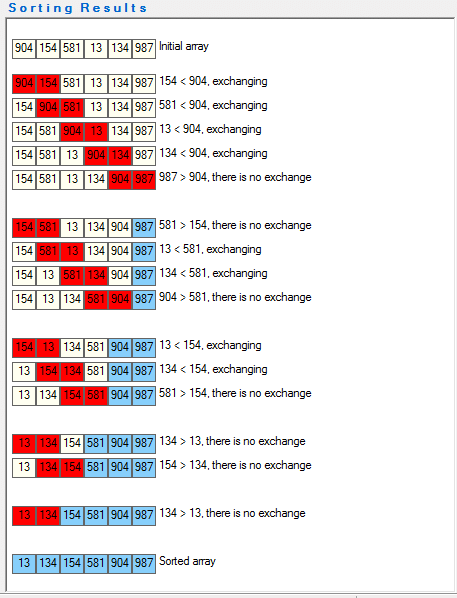
\includegraphics[scale=0.5]{img/Obtained-result-using-Bubble-sort-algorithm-and-array-with-six-elements.png}
    \caption{Corrida de Bubble Sort para un arreglo no ordenado (imagen sacada de Google).}
\end{figure}

A continuación, el código para el algoritmo de la burbuja\marginfootnote{Pseudocódigo sacado del Cormen.}:

\begin{algoritmo}
    \caption{Bubble Sort}\label{alg:bubble}
    \KwData{$A$ arreglo no ordenado}
    \KwResult{$A$ arreglo ordenado}
    \For{$i \leftarrow 1$ \textup{hasta} $length[A]$}{
        \For{$j \leftarrow length[A]$ \textup{hasta} $i+1$}{
        \If{$A[j] < A[j-1]$}{
        intercambia $A[j] \rightleftarrows A[j-1]$
        }
        }
    }
\end{algoritmo}

\break

Analicemos el algoritmo. Las operaciones son comparaciones e intercambio de valores. Así que, si el conjunto tiene $n$ elementos y esa es la medida de la instancia:

\begin{itemize}
    \item Para cada $j$ se hacen $n - j - 1$ comparaciones.
    \item Son $(n-1) + (n-2) + \dots + 2 + 1 = \frac{1}{2}n(n-1)$.
    \item Esto es $O(n^2)$.
    \item La cantidad de intercambios es también $O(n^2)$ (esto en el peor de los casos, se hace un intercambio después de cada comparación).
\end{itemize}

\textbf{En conclusión:} El algoritmo de la burbuja tiene eficiencia $O(n^2)$ en función de la cantidad de elementos del conjunto a ordenar.

Comparemos el algoritmo de la burbuja con una versión del algoritmo de inserción. El \textbf{algoritmo de inserción} construye una lista comenzando con el primer elemento del conjunto dado. Luego agrega el segundo elemento a la lista \textit{en el lugar correcto}. Y así sigue con los demás elementos del conjunto de manera que cada lista queda ordenada de una vez. La eficiencia de este algoritmo depende del método que se utilice para insertar el elemento \textit{en el lugar correcto}.

En nuestro caso, usaremos el método de \textbf{bisección}: Para insertar el $i$-ésimo elemento, se decide en cuál mitad de la lista debería ir. Después, en cuál mitad de esa mitad debería ir y así sucesivamente.

Ahora, analicemos este algoritmo:

\begin{itemize}
    \item Supongamos que el conjunto a ordenar tiene $n$ elementos.
    \item Si $n$ está entre $2^{r-1}$ y $2^r$, entonces hay que hacer $r$ comparaciones.
    \item En total son $\log_22 + \log_23 + \dots + \log_2 n$ comparaciones (aprox.).
    \item Esto es $O(n\log n)$.
\end{itemize}

\textbf{En conclusión}: El algoritmo de inserción, usando el método de bisección tiene eficiencia $O(n \log n)$. Pero al hacer la inserción en el lugar correcto, en el peor de los casos hay que intercambiar los términos de la lista. Esto serían otra vez $n^2$ intercambios. Por tanto, este algoritmo tiene también eficiencia $O(n^2)$.